% Change to use the correct class file for your paper.
\documentclass{sig-alternate-10pt}[10]

%\pagenumbering{arabic}
\usepackage{pbox}
\usepackage{pifont}
\usepackage{multirow}
\usepackage{amsfonts}     % Adds math fonts, commands such as \begin{align}
\usepackage{array}        % Tables for use in math mode
\usepackage{booktabs}     % Elegant table-formatting library
\usepackage{bold-extra}   % Provides bf+sc (only in textbf+textsc env.)
\usepackage[skip=5pt]{caption}
\usepackage{color}        % Allow the use and definition of colors
\usepackage{colortbl}     % Color table cells
\usepackage{comment}      % Provides \begin,\end{comment} for large blocks
\usepackage{endnotes}     % Footnotes pushed to the end of a document
\usepackage{gensymb}      % Adds useful symbols w/out math mode, e.g. \degree
\usepackage{graphicx}     % For importing graphics
\usepackage{hyperref}     % Creates hyperlinks from ref/cite 
\hypersetup{pdfstartview=FitH}
\usepackage{listings}     % in-line source code (poorly, consider minted)
\usepackage{multirow}     % Multiple row spacing in tables
\usepackage{nth}          % Typeset 33rd correctly as \nth{33}
%\usepackage[section]{placeins} % Don't let figs escape their sections
\usepackage{rotating}     % Rotates any object, note sideways != sidewaysfigure
%\usepackage[all=normal]{savetrees} % For when space is tight, read manual and
                          % selectively enable things. CAN BREAK CONF STYLES!!
\usepackage{soul}         % Provides \hl{} for highlighting
%\usepackage{subfig}
%\usepackage{subfigure}    % Complicated figure creation
%\usepackage{subcaption}   % Replaces both subfig and subfigure
\usepackage[nofancy]{svninfo} % svn information in docs (req. svn:keywords)
\usepackage{tabularx}     % Complicated table creation
\usepackage{threeparttable} % Add footnotes to a table
\usepackage{units}        % For nice fractions, \nicefrac{1}{2} --> 1/2
\usepackage{url}          % Pretty printing of hyperlinks
\usepackage{xspace}       % Intelligently add spaces after commands
\usepackage{times}
\usepackage{breakurl}
\usepackage{epsfig}
\usepackage{subfigure}
\usepackage{epstopdf}

%\DeclareCaptionType{copyrightbox}

%\newlength\SUBSIZE

\columnseprule 0pt
\renewcommand{\arraystretch}{1.2} % Space out rows in tables
\renewcommand{\paragraph}[1]{\noindent \textbf{#1}\ \ \ \ }

\newcommand{\PERFSENSE}{$\sf\small{PerfSense}$\xspace}
\newcommand{\UMICH}{$\sf\small{UMICH}$\xspace}
\newcommand{\UMICHLTE}{$\sf\small{UMICH\-LTE}$\xspace}
\newcommand{\RC}{$\small{\textbf{\texttt{RRC\_CONNECTED}}}\normalsize$\xspace}
\newcommand{\RI}{$\small{\textbf{\texttt{RRC\_IDLE}}}\normalsize$\xspace}
\newcommand{\RCB}{${\textbf{\texttt{RRC\_CONNECTED}}}\normalsize$\xspace}
\newcommand{\RIB}{${\textbf{\texttt{RRC\_IDLE}}}\normalsize$\xspace}
\newcommand{\FT}{$\sf\small{4GTest}$\xspace}
\newcommand{\TT}{$\sf\small{3GTest}$\xspace}

\newcommand{\IGL}{\includegraphics[width=0.995\textwidth]}
\newcommand{\IG}{\includegraphics[width=0.3\textwidth]}
\newcommand{\IGML}{\includegraphics[width=0.47\textwidth]}
\newcommand{\IGMM}{\includegraphics[width=0.385\textwidth]}
\newcommand{\IGM}{\includegraphics[width=0.27\textwidth]}
\newcommand{\IGS}{\includegraphics[width=0.23\textwidth]}

\newcommand{\mycomment}[1]{{\color{red}[\textsf{#1}]}}
\newcommand{\alfred}[1]{\textcolor{red}{\cut{[Alfred: #1]}}}
\newcommand{\cut}[1]{}
\newcommand{\umichauthor}{{\%}}
%\setlength\paperheight {11in}
%\setlength\paperwidth {8.5in}

% Set the graphics path
\graphicspath{{../figs/}{../images/build/}}

% No space between bibliography items:
\let\oldthebibliography=\thebibliography
  \let\endoldthebibliography=\endthebibliography
  \renewenvironment{thebibliography}[1]{%
    \begin{oldthebibliography}{#1}%
      \setlength{\parskip}{0ex}%
      \setlength{\itemsep}{0ex}%
  }%
  {%
    \end{oldthebibliography}%
  }
\setlength{\parindent}{5mm}

\begin{document}

\title{VoLTE Data Free-Ride Attack: A Case of Exploiting the Unprotected Voice Channel}
\author{
Yunhan Jack Jia, Qi Alfred Chen, Z.~Morley Mao,\\
Alex Yoon$^\dagger$, Jie Hui$^\dagger$, Salvador Mendoza, Samson Kwong$^\dagger$, Kevin Lau$^\dagger$,Kranthi Sontineni$^\dagger$,
\\
University of Michigan, $^\dagger$T-Mobile USA Inc.
\\
%\{jackjia, alfchen, zmao\}@umich.edu,\\ $^\dagger$\{alex.yoon4, jie.hui, salvador.mendoza12, samson.kwong, kevin.lau, kranthi.sontineni1\}@t-mobile.com
} 
\iffalse
\numberofauthors{2}
\author{
\small{
    \alignauthor Yunhan Jack Jia, Qi Alfred Chen, and Z.~Morley Mao \\
    \affaddr{University of Michigan} \\
    %\email{\{jackjia, alfchen, zmao\}@umich.edu}
    \alignauthor Alex Yoon, Jie Hui, Salvador Mendoza, Samson Kwong, Kevin Lau, Kranthi, Sontinei \\
    \affaddr{T-Mobile USA Inc.$^1$}\\
    %\email{\{alex.yoon4, jie.hui, salvador.mendoza12, samson.kwong, kevin.lau, kranthi.sontineni1,\}@t-mobile.com}
}}
\fi
\iffalse
\numberofauthors{8}
\author{
\alignauthor
Yunhan Jack Jia \\
	\affaddr{University of Michigan} \\
	\email{\normalsize alfchen@umich.edu} \\
\alignauthor
Qi Alfred Chen \\
	\affaddr{University of Michigan} \\
	\email{\normalsize alfchen@umich.edu} \\
\alignauthor
Z.~Morley Mao \\
	\affaddr{University of Michigan} \\
	\email{\normalsize haokun@umich.edu} \\
\alignauthor
Jie Hui \\
	\affaddr{University of Michigan} \\
	\affaddr{Ann Arbor, MI} \\
	\email{\normalsize sanae@umich.edu} \\
\alignauthor
Z. Morley Mao \\
        \affaddr{University of Michigan} \\
        \affaddr{Ann Arbor, MI} \\
	\email{\normalsize zmao@umich.edu} \\
\and
\alignauthor
Jie Hui \\
        \affaddr{T-mobile} \\
        \affaddr{Seattle, WA} \\
        \email{\normalsize jie.hui@t-mobile.com} \\
\alignauthor
Karthik Iyer \\
        \affaddr{T-mobile} \\
        \affaddr{Seattle, WA} \\
        \email{\normalsize karthik.iyer@t-mobile.com} \\
\alignauthor
Kevin Lau \\
        \affaddr{T-mobile} \\
        \affaddr{Seattle, WA} \\
        \email{\normalsize kevin.Lau@t-mobile.com} \\
}
\fi

%\conferenceinfo{EECS 582 -- Winter'13} {Jan 10--Apr 23, 2013, Ann Arbor, Michigan, USA.}
%\CopyrightYear{2013}
%\crdata{XXX-X-XXXXX-XXX-X}

\maketitle

\cut{
%don't need this line for now since it is double-blind in submission
\footnotetext[1]{The views presented in this paper are as individuals and do not necessarily reflect any position of T-Mobile.} 
}

% ABSTRACT

% Write abstract here.
% Header information is handled by \LaTeX{} magic.

\section{Introduction}
%new version, from Alfred

Mobile data is charged according to the traffic volume, while the voice call is usually charged by the call duration. We find that an emerging telephony service, Voice over LTE (VoLTE), introduces critical problem to the current billing system deployed in the cellular network: it allows fraudulent users to utilize high-speed LTE data \emph{for free} by transmitting data using the voice channel dedicated to VoLTE. Compared with the ``toll-free'' data access attacks proposed by previous work~\cite{peng2012mobile,go2014gaining} that rely on spoofing or the assumption that operators don't charge specific types of traffic (e.g., DNS, TCP retransmission), the data free-ride attack leverages the inconsistency between operators' charging policies for voice and data.

We successfully implement this attack using ICMP tunnel between a device and a proxy server, which can fetch content from the Internet for free with up to 7 Mbps bandwidth. We verify that this problem affects at least two of the major operators in the US. We attribute this problem to the lack of access control of network interfaces dedicated to VoLTE on both device and network sides, and are working with one of the operators to deploy mitigation countermeasures against such attack. 

%\category{C.2.1}{COM\-PU\-TER-COM\-MU\-NICATION
%  NET\-WORKS}{Network Architecture and Design}[Wireless communication]
%\category{B.8.0}{HARD\-WARE}{Performance and Reliability}[General]
%\terms{Design, Experimentation, Measurement, Performance}
%\keywords{Cellular, Mobile, Throughput, Energy, Context, Prediction, LTE, HSPA}

%\newpage

% page limit          % 14.0 pg
% abstract            %  0.5 pg
%\vfill\eject
\section{Data Free-ride Attack}
\label{sec:intro}
%new version, from Alfred
VoLTE transmits voice data over LTE network and through the IP Multimedia Subsystem (IMS) cores using a ``dedicated bearer'', which is a ``pipe line'' that transports data between the device and the gateways. Prior to VoLTE, all the application data is transmitted by a default bearer where QoS is not guaranteed.

\textbf{Attack Design. }Shown in Fig 1, the two different bearers are implemented as two network interfaces on Android device, denoted as \texttt{IF0} for default bearer and \texttt{IF1} for dedicated bearer. Using which interface to send a certain packet flow is controlled by the routing table on the device, where \texttt{IF0} is set to be used by default and \texttt{IF1} is used when the destination of the packets is the IMS nodes. We discovered that user with root privilege can send packets to arbitrary destinations using \texttt{IF1} by manipulating the routing table. These packets sent from \texttt{IF1} bypass the volume-based charge since they are carried by the voice channel, and also won't incur any time-based charge because no call session is initiated. We also unrevealed that downlink ICMP packets can be sent to \texttt{IF1} from third-party servers without getting blocked by the firewall or incurring any charge, which grants fraudulent user free uplink and downlink data access. User can thus set up their own proxy to intercept device's HTTP request sent from \texttt{IF1}, fetch contents from the Internet and transmit data back to the \texttt{IF1} on the device using an ICMP tunnel free of charge. 

\textbf{Validation. }We have built a demo app to show the feasibility of downloading a 10 MB video within 2 seconds free of data charge from the proxy server outside the cellular network and we measured that the downlink bandwidth of this free data channel can be up to 7 Mbps! 

\begin{figure}[!t]
\hspace{-0.2in}
\centering
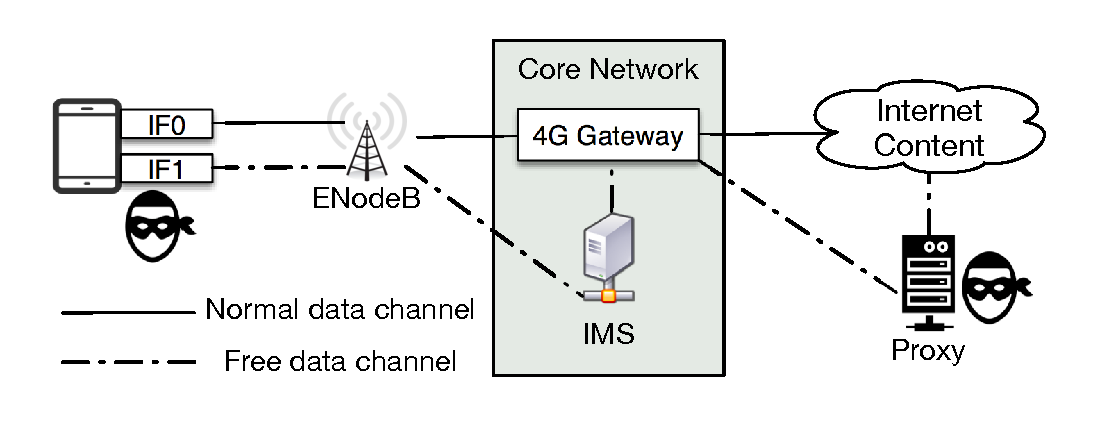
\includegraphics[width=3.3in]{figs/poster.eps}
\caption{VoLTE Data free ride attack.}
\vspace{-0.1in}
\label{fig:attack}
\end{figure}
         % 1.5 pg
\section{Mitigations}
\label{sec:background}
\textbf{Network side mitigation. }Considering that the dedicated bearer is supposed to only talk directly with the internal IMS nodes, we have worked with one of the operators to apply additional traffic blocking rules on the packet gateway to block the packets that have external IP address as their source or destination addresses from using IMS APN, which prevents \texttt{IF1} from forwarding traffic to attacker controlled servers and protects it from unsolicited traffic. We evaluate this countermeasure in the experimental environment and verify that it blocks the free data-ride without affecting other services. However, this approach only blocks the ICMP tunnel towards\texttt{IF0}, and other protocols may also be abused to conduct data free-ride attack.\cut{In addition, we suggest operators to limit the bandwidth for the dedicated bearer in order to mitigate the potential threat of abuse, since there is no valid reason to allocate bandwidth for VoLTE that far exceeds its requirement.} 

\textbf{Device side mitigation. }The lack of access control of network interfaces on the device is inherited from the Linux kernel, where privileged user is allowed to change the routing table. We suggest migrating sensitive functionalities such as forwarding rules to a trusted space (e.g., TrustZone~\cite{trustzone}), which can prevent it from manipulation from untrusted sources.

%Uncomment this line if your paper has / uses end notes
%\theendnotes

{
\footnotesize
\raggedright
\bibliographystyle{abbrv}
\bibliography{paper}
}

%\input{title}


\end{document}

